% chapter4.tex -- Distinction of Our Naming of GS from the Original Paper
% Based on the author's UGThesis.docx.

\chapter{Distinction of Our Naming of the Generating Set from the Original Paper}
\label{ch:gs_distinction}

In this chapter we clarify an important difference between the definition of generating chords used in the original paper by Parvez, Rahman, and Nakano~\cite{parvez2011} and the definition we adopt in this thesis. 
This distinction is necessary for the introduction of the \emph{valid generating set} (VGS) in later chapters, which allows us to handle multi‑edge conflicts in biconnected graphs.

\section{Original Definition}
\label{sec:original_gs}

In the original paper~\cite{parvez2011}, a chord \((v_1, v_j)\) of a triangulation \(T\) (with root vertex \(v_1\)) is called a \textbf{generating chord} if flipping it produces a child triangulation \(T'\) whose leftmost blocking chord is exactly the newly added chord. 
Only chords that satisfy this property are included in the generating set \(GS\). 
As shown in Chapter~\ref{ch:cycle_algorithm}, this condition is equivalent to requiring that the other endpoint \(j\) be at least \(b'\), where \((v_b, v_{b'})\) is the leftmost blocking chord of \(T\) (or \(j \ge 3\) for the root).

Thus, in the original algorithm, \(GS\) is a subset of the chords incident to the root, and its size varies with the triangulation.

\section{Our Definition}
\label{sec:our_gs}

In contrast, for the purpose of handling biconnected graphs, we define the \textbf{generating set} \(GS\) more broadly:

\begin{definition}[Our generating set]
    \label{def:our_gs}
    For a triangulation \(T\) of a cycle with root vertex \(v_1\), the set \(GS\) consists of \emph{all} chords that have \(v_1\) as one endpoint, i.e., all chords of the form \((v_1, v_j)\) for \(j = 3, 4, \dots, n-1\) that are present in \(T\). 
    No further restriction is applied.
\end{definition}

In other words, every chord incident to the root is considered a \emph{generating chord} in our terminology, regardless of whether flipping it would yield a child whose leftmost blocking chord is the new chord.

\section{Why This Distinction Is Necessary}
\label{sec:why_distinction}

The broader definition is needed for the construction of the \textbf{valid generating set} (VGS) introduced in Chapter~\ref{ch:vgs}. 
In the biconnected case, some chords incident to the root, when flipped, may create a multi‑edge conflict with chords from previously processed faces. 
To avoid generating invalid triangulations, we must identify which generating chords are \emph{safe} to flip. 
The VGS will contain exactly those chords \((v_1, v_j)\) whose flip does not introduce a multi‑edge.

If we had used the original, more restrictive definition of generating chords, we would lose the ability to control safety via a simple subset. 
By including all root‑incident chords in \(GS\), we can later filter them based on multi‑edge checks, resulting in the VGS. 
The original condition (whether the flipped chord becomes the leftmost blocking chord) remains relevant for the correctness of the genealogical tree, but it is applied separately when we actually perform the flip.

\section{Flippability Condition for Our GS}
\label{sec:flippability_condition}

Even though we call all root‑incident chords ``generating'', not every such chord can be flipped while preserving the parent‑child relationship defined in Chapter~\ref{ch:cycle_algorithm}. 
For a chord \((v_1, v_j)\) to be flipped and produce a child triangulation whose parent is the current one, we must still ensure that the flipped chord becomes the leftmost blocking chord of the child. 
This condition, as proved in the original paper, is \(j \ge b'\), where \((v_b, v_{b'})\) is the leftmost blocking chord of the current triangulation (with \(b < b'\)).

We now restate and prove this condition in a self‑contained manner, following the author’s original argument.

\begin{lemma}[Flippability condition]
    \label{lem:flippability_condition}
    Let \(T\) be a triangulation of a cycle with root vertex \(v_1\). 
    Let \((v_b, v_{b'})\) be the leftmost blocking chord of \(T\) (if \(T\) is the root, we set \(b' = 2\) for convenience). 
    Then flipping a chord \((v_1, v_j)\) in \(T\) yields a child triangulation \(T'\) for which \(T\) is the parent if and only if \(j \ge b'\).
\end{lemma}

\begin{proof}
    We consider two cases based on the value of \(j\) relative to \(b'\).

    \begin{figure}[htbp]
        \centering
        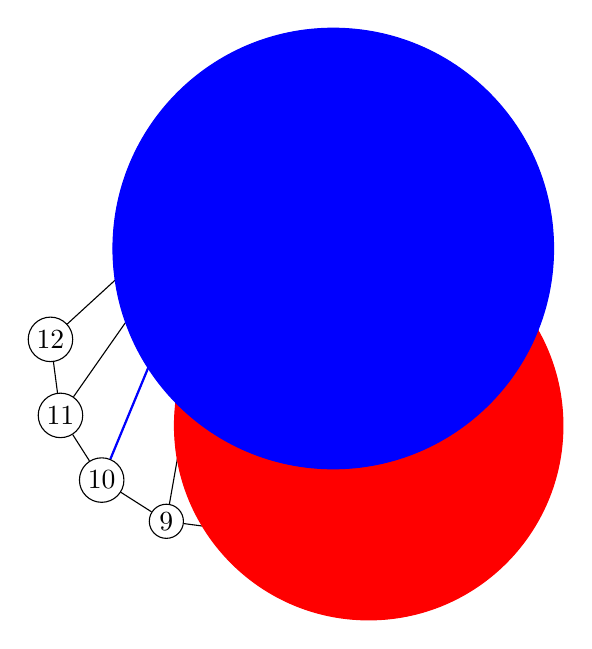
\begin{tikzpicture}[scale=0.9, every node/.style={circle, draw, fill=white, inner sep=1.5pt}]
            % Vertices arranged in a circle
            \foreach \i/\angle in {1/90,2/65,3/40,4/15,5/-10,6/-35,7/-60,8/-85,9/-110,10/-135,11/-160,12/175} {
                \node (v\i) at (\angle:2.5) {\i};
            }
            \draw (v1)--(v2)--(v3)--(v4)--(v5)--(v6)--(v7)--(v8)--(v9)--(v10)--(v11)--(v12)--(v1);
            % Root chords
            \draw (v1)--(v3);
            \draw (v1)--(v4);
            \draw (v1)--(v5);
            \draw (v1)--(v7);
            \draw (v1)--(v8);
            \draw (v1)--(v9);
            \draw (v1)--(v10);
            \draw (v1)--(v11);
            % Blocking chords
            \draw[red, thick] (v4)--(v7);
            \node at (0,0) {\(v_1\)};
            \node[red] at (2, -1) {leftmost blocking chord \((v_4, v_7)\)};
            \node[blue] at (1.5, 1.5) {generating chord \((v_1, v_j)\) with \(j \ge 7\)};
            \draw[blue, thick] (v1)--(v10);
        \end{tikzpicture}
        \caption{Illustration of the leftmost blocking chord \((v_b, v_{b'}) = (v_4, v_7)\) and a generating chord \((v_1, v_{10})\) with \(j = 10 \ge 7\).}
        \label{fig:flippability}
    \end{figure}

    \noindent\textbf{Case 1: \(j < b'\).} 
    Assume \(j < b'\). 
    The chord \((v_1, v_j)\) lies entirely to the left of the leftmost blocking chord \((v_b, v_{b'})\) when we walk clockwise from \(v_1\) along the cycle. 
    Flipping \((v_1, v_j)\) replaces it with a chord \((v_p, v_q)\) where both endpoints lie between \(v_j\) and the opposite side of the quadrilateral. 
    Because \(j < b'\), the new chord \((v_p, v_q)\) will have its larger endpoint at most \(b'\). 
    Consequently, the leftmost blocking chord of the resulting triangulation remains \((v_b, v_{b'})\) (or another chord with the same larger endpoint \(b'\)). 
    Thus the flipped chord is not the leftmost blocking chord of the child, and the parent of the child would not be \(T\). 
    Hence \((v_1, v_j)\) is not flippable in the sense that it does not preserve the parent‑child relationship.

    \noindent\textbf{Case 2: \(j \ge b'\).} 
    Now assume \(j \ge b'\). 
    Consider the quadrilateral formed by \(v_1, v_{b}, v_{b'}, v_j\) (or a suitable quadrilateral if \(j > b'\)). 
    Flipping \((v_1, v_j)\) removes it and adds the opposite diagonal \((v_{b}, v_{p})\) for some \(p\) with \(p > b'\) (if \(j = b'\)) or a chord \((v_{q}, v_{r})\) with larger endpoints than \(b'\). 
    In all subcases, the newly added chord has its larger endpoint strictly greater than \(b'\). 
    Therefore it becomes the new leftmost blocking chord of the child triangulation. 
    By definition, \(T\) is the parent of this child, so \((v_1, v_j)\) is flippable and preserves the tree structure.
\end{proof}

\begin{remark}
    For the root triangulation, there is no blocking chord; we set \(b' = 3\) (the smallest index of a chord incident to \(v_1\)). 
    Then the condition \(j \ge 3\) holds for every chord \((v_1, v_j)\) with \(j \ge 3\), so all such chords are flippable, which matches the fact that the root has \(n-3\) children.
\end{remark}

\section{Implication for Our Algorithm}
\label{sec:implication}

In the original paper, the generating set \(GS\) is defined as exactly the set of flippable chords (those with \(j \ge b'\)). 
Thus, when the algorithm traverses the genealogical tree, it iterates directly over \(GS\).

In our work, we define \(GS\) as \emph{all} chords incident to the root, which is a superset of the flippable chords. 
When we need to generate children, we must still restrict to those with \(j \ge b'\). 
However, we also need to check an additional condition: whether flipping the chord would create a multi‑edge with chords from previously processed faces (in the biconnected setting). 
Therefore we maintain a separate \textbf{valid generating set} (VGS) that contains exactly those chords \((v_1, v_j)\) satisfying:

\begin{enumerate}
    \item \(j \ge b'\) (flippability condition), and
    \item The opposite pair of \((v_1, v_j)\) is not already present in the global chord set \(S\) (safety condition).
\end{enumerate}

This distinction is crucial for the pruning strategy described in Chapter~\ref{ch:pruning_strategy} and for maintaining \(O(1)\) amortised time per triangulation.

\section{Summary}
\label{sec:gs_summary}

We have clarified the difference between the original definition of generating chords and our broader definition. 
The broader definition allows us to later filter chords based on multi‑edge conflicts, leading to the concept of a valid generating set. 
The flippability condition \(j \ge b'\) remains essential for preserving the parent‑child relationship in the genealogical tree. 
This condition is used in our algorithm when iterating over candidate chords to flip.